\documentclass[11pt]{article}
\usepackage{amsmath,amssymb,amsthm}
\usepackage[utf8]{inputenc}
\usepackage[T1]{fontenc}
\usepackage{lmodern}
\usepackage{geometry}
\usepackage{tabularx}
\usepackage{graphicx}
\usepackage{hyperref}
\usepackage{orcidlink}
\usepackage{enumitem}
\usepackage{graphicx}
\usepackage{tikz}
\usepackage{color}
\usepackage{booktabs}
\usepackage{pgfplots}
\pgfplotsset{compat=1.18}
\geometry{margin=1in}
\hypersetup{
	colorlinks=true,
	linkcolor=blue!60!black,
	citecolor=blue!60!black,
	urlcolor=blue!60!black
}


\newtheorem{theorem}{Theorem}[section]
\newtheorem{lemma}[theorem]{Lemma}
\newtheorem{proposition}[theorem]{Proposition}
\newtheorem{corollary}[theorem]{Corollary}
\theoremstyle{definition}
\newtheorem{definition}[theorem]{Definition}
\newtheorem{remark}[theorem]{Remark}
\newtheorem{assumption}[theorem]{Assumption}

\begin{document}
    \title{\textbf{Macroscopic Tunnelling and Resonances in Spectral Geometry:}\\ Agmon–Weitzenböck Bounds and the \(\rho\)-Intensity Unification}
    
	\author{Mohamed H. M. Makraini\,\orcidlink{0009-0007-6597-3283}\\
		\small UNED National University, Madrid\\
		\small \texttt{mhamed34@alumno.uned.es}}
	\date{October 10, 2025}
	\maketitle
	
	\begin{abstract}
		We develop a physics-first account of macroscopic quantum tunnelling through the lens of spectral geometry. Our framework treats tunnelling exponents, resonance localization, and stability of scalar excitations within a single, density-weighted spectral setting. We prove sharp exponential bounds for transmission, establish resonance poles through complex scaling with controlled widths, and show that a weighted Weitzenböck inequality yields a positive lower bound for the relevant spectral operator—an effect we term ``spectral confinement.'' Two case studies illustrate the reach of the approach: (i) escape rates in a Josephson “washboard” potential consistent with mesoscopic experiments, and (ii) shape and Aharonov–Bohm resonances where the spectral weight governs both localization and linewidths. As an outlook, we argue that the same spectral mechanism that organizes macroscopic tunnelling can act as a protective principle for scalar masses, avoiding ad hoc fine-tuning. All results come with a minimal, reproducible pipeline (notebooks and tables) to enable verification and reuse. This positions spectral geometry as a unifying language from chip-scale quantum phenomena to field-theoretic stability questions.
		\textit{Context:} The 2025 Nobel Prize in Physics recognized macroscopic quantum mechanical tunnelling and energy quantization in superconducting circuits, underscoring the timeliness of a unified spectral treatment. ([NobelPrize.org][1])
	\end{abstract}
	
	\noindent{\bf Keywords:}
	spectral geometry; non-commutative geometry; twistor geometry; Higgs hierarchy; spectral gap; Bakry–Émery curvature; spectral action.
	
	\section*{Executive Overview}
	
	\paragraph{Motivation and context.}
	Macroscopic quantum tunnelling and energy quantization in superconducting circuits have moved quantum phenomena firmly into the mesoscopic--macroscopic regime. This work leverages that momentum to formulate a unified, density–weighted spectral geometry that simultaneously explains tunnelling exponents, resonance localization, and scalar-mode stability (``\textbf{spectral confinement}'').
	
	\paragraph{Contributions.}
	\begin{enumerate}[label=(\roman*)]
	\item A rigorous spectral–geometric bound for tunnelling probabilities based on Agmon-type decay with an explicit geometric weight; 
	\item a resonance framework via complex scaling that controls pole locations and widths in terms of the same weight;
	\item a weighted Weitzenböck positivity inequality delivering a nonzero spectral gap (``\textbf{spectral confinement}'') for the positive representative of the Dirac-type operator; 
	\item a reproducible pipeline (analytic lemmas + numerical notebooks) validating benchmark barriers and mesoscopic circuits.
	\end{enumerate}
	\paragraph{Main results (citable).}
	\begin{itemize}
		\item \textbf{Agmon–weighted tunnelling:} sharp exponential transmission bounds derived from a geometry-induced distance, with constants tracked for benchmark potentials.
		\item \textbf{Resonances via complex scaling:} meromorphic continuation yields poles whose real parts and widths are controlled by the geometric weight; applicability to shape and Aharonov--Bohm scenarios.
		\item \textbf{Weitzenböck positivity \(\Rightarrow\) spectral confinement:} a lower bound on the positive spectral representative implies robust localization of scalar modes.
	\end{itemize}
	
	\paragraph{Case studies.}
	\emph{(I) Josephson washboard.} Predicted escape rates match mesoscopic operating regimes and illustrate how the spectral weight governs both exponent and prefactor. 
	\emph{(II) Shape/AB resonances.} Pole patterns and linewidths follow from the same geometric control, providing a unified interpretation across magnetic and topological settings.
	
	\paragraph{Predictions and outlook.}
	The framework anticipates (a) resonance towers with spacing governed by the geometric weight, and (b) small, universal deviations in effective parameters at large curvature scale. As an outlook, we discuss how the same confinement mechanism can act as a protective principle for scalar masses, without elevating this to a central claim here.
	
	\paragraph{Reproducibility.}
	All figures and tables are generated from notebooks and scripts provided with the submission (barrier benchmarks, washboard escape, resonance localization), enabling independent verification and reuse.
	
	
	\section{Main Results}
	\label{sec:main-results}
	
	\paragraph{Standing hypotheses.}
	Let $(M,g)$ be a smooth time-slice (or a Riemannian manifold after OS$_2$) equipped with a density field $p = e^{-2\phi}$, $\phi\in C^\infty(M)$, and a Dirac-type operator $D$ acting on a Hermitian/Krein bundle $\mathcal{K}\to M$.
	Write $E(D):=(D^\dagger D)^{1/2}$ for the positive representative.
	We assume:
	\begin{itemize}
		\item[(H1)] (\emph{Weighted Weitzenböck identity}) $D^2=\nabla_\phi^\ast\nabla_\phi+R_\phi$ as quadratic forms on $\mathrm{Dom}(D^2)$, with $R_\phi$ an endomorphism (``effective curvature'').
		\item[(H2)] (\emph{Bakry--Émery lower bound}) $R_\phi \ge K_\ast\,\mathrm{Id}$ in the sense of forms, for some $K_\ast\in\mathbb{R}$ on the region of interest.
		\item[(H3)] (\emph{Regularity/size of the weight}) $\nabla\phi\in L^\infty_{\mathrm{loc}}$, and on the relevant domain $\|\nabla\phi\|_\infty<\infty$; boundary condition is Dirichlet at the locus $\rho=0$ (if present).
		\item[(H4)] (\emph{Semiclassical window for tunnelling}) There is a small parameter $h\in(0,h_0]$ (e.g. effective $\hbar$ or inverse mass) and an energy $E$ below the top of the barrier; the \emph{Agmon functional} $S_p(E)$ is finite (defined below).
		\item[(H5)] (\emph{Stability}) Internal fluctuations are $D$-bounded with relative bound $<1$ (Kato--Rellich); OS$_2$ reflection positivity holds for the physical sector.
	\end{itemize}
	
	\paragraph{Agmon geometry with $\rho$-weight.}
	Let $W_p(\cdot;E)\ge 0$ denote a (problem-dependent) forbidden-energy density induced by the pair $(\rho,E)$
	(e.g. the positive part of an effective potential in the $p$-weighted metric/cometric).
	Define the $\rho$-Agmon distance by
	\[
	\mathrm{dist}_{\mathrm{Ag},\rho}(x,y;E)
	:= \inf_{\gamma}\int_\gamma \sqrt{W_p(\gamma(s);E)}\,\mathrm{d}s,
	\]
	and the \emph{Agmon action} across the barrier by
	\[
	S_p(E):=\inf_{\Gamma}\int_{\Gamma}\sqrt{W_p(\xi;E)}\,\mathrm{d}s,
	\]
	where the infimum runs over curves $\Gamma$ connecting classically allowed components at energy $E$.
	
	\begin{theorem}[Agmon--$\rho$ tunnelling bound]\label{thm:agmon-rho}
		Assume \textup{(H1)--(H4)}. Then there exist $c_\pm>0$ and $h_0>0$ (depending on geometric data, on $W_p$, and on the barrier geometry) such that for all $0<h\le h_0$ and all energies $E$ in the tunnelling window,
		\[
		c_-\,h^{\alpha}\,e^{-\tfrac{2}{h}S_p(E)} 
		\;\le\; \mathsf{T}(E;h) 
		\;\le\; c_+\,h^{\beta}\,e^{-\tfrac{2}{h}S_p(E)}.
		\]
		Here $\mathsf{T}(E;h)$ is the transmission probability, while $\alpha,\beta$ are barrier-dependent rational exponents (coming from transport equations for the WKB prefactor).
		In particular,
		\[
		-\frac{h}{2}\log \mathsf{T}(E;h)\;=\; S_p(E)\,+\,\mathcal{O}(h\log h^{-1}).
		\]
		\emph{Sharpness.} If the turning set is nondegenerate and $W_p$ is smooth with a unique minimising geodesic for $S_p(E)$, the exponents $\alpha,\beta$ and prefactors $c_\pm$ are computable from transport equations along that geodesic.
	\end{theorem}
	
	\begin{theorem}[Weitzenböck-gap $\Rightarrow$ spectral confinement]\label{thm:weitzenbock-gap}
		Assume \textup{(H1)--(H3)} with $K_\ast>0$ on a connected region $\Omega\subseteq M$ and Dirichlet boundary at $\partial\Omega\cup\{\rho=0\}$. Then there exists a constant $C_d>0$, depending only on the local dimension, ellipticity constants, and geometry of $(\Omega,g,\phi)$, such that the first positive eigenvalue of $E(D)^2$ obeys
		\[
		\lambda_1\big(E(D)^2\vert_{\,\Omega}\big)\;\ge\; K_\ast \;-\; C_d\,\|\nabla\phi\|_{L^\infty(\Omega)}^{2}.
		\]
		Consequently, if $K_\ast - C_d\|\nabla\phi\|_\infty^{2}>0$, the spectrum of $E(D)^2$ on $\Omega$ has a strictly positive gap at the origin.
		We refer to this effect as \emph{spectral confinement}.
	\end{theorem}
	
	\begin{corollary}[Resonances: location and widths]\label{cor:resonances}
		Under \textup{(H1)--(H5)}, suppose the coefficients are analytic outside a compact set so that complex scaling by an angle $\theta\in(0,\theta_0)$ yields a non-selfadjoint deformation with meromorphic resolvent.
		Then the deformed operator admits a discrete set of poles $(z_j)_{j\in J}$, $z_j=E_j - \tfrac{i}{2}\Gamma_j$, and there exist constants $A,B>0$ (geometry-dependent) with
		\[
		0<\Gamma_j \;\le\; A\,h^{B}\,e^{-\tfrac{2}{h}S_p(E_j)}.
		\]
		In particular, the same $\rho$-Agmon action that governs tunnelling controls the resonance widths; stronger $\rho$-gradients (larger $\|\nabla\phi\|$) shrink $\Gamma_j$ within the validity window.
	\end{corollary}
	
	\begin{remark}[On hypotheses and sharpness]
		\leavevmode
		\begin{enumerate}
			\item The constant $C_d$ in Theorem~\ref{thm:weitzenbock-gap} depends only on local analytic bounds and dimensional constants (no global fine-tuning).
			\item For multi-well geometries, $S_p(E)$ is the minimum over all connecting geodesics; interference effects modify prefactors but not the leading exponential.
			\item Magnetic/topological settings (Aharonov--Bohm, shape resonances) fit Corollary~\ref{cor:resonances} provided analyticity of coefficients holds on the scaled sector; the $\rho$-weight enters the Agmon density $W_p$ through the effective symbol.
		\end{enumerate}
	\end{remark}
	
	\paragraph{Validity range and hypotheses at a glance.}
	\begin{center}
		\small
		\begin{tabular}{p{0.18\linewidth} p{0.35\linewidth} p{0.38\linewidth}}
			\toprule
			\textbf{Result} & \textbf{Key hypotheses} & \textbf{Validity / notes} \\
			\midrule
			Theorem~\ref{thm:agmon-rho} (Agmon--$\rho$) 
			& (H1)--(H4); smooth barrier; nondegenerate turning set; finite $S_p(E)$
			& $0<h\le h_0$; leading exponential exact; prefactors from transport; multi-path interference affects only $c_\pm,h$-powers \\[4pt]
			Theorem~\ref{thm:weitzenbock-gap} (Gap)
			& (H1)--(H3); $R_\phi\ge K_\ast>0$; $\|\nabla\phi\|_\infty<\infty$; Dirichlet at $\rho=0$
			& Local gap if $K_\ast>C_d\|\nabla\phi\|_\infty^2$; constants independent of global cutoffs \\[4pt]
			Cor.~\ref{cor:resonances} (Resonances)
			& (H1)--(H5); exterior analyticity; admissible complex scaling
			& Poles $z_j$ with widths $\Gamma_j\lesssim h^{B}e^{-2S_p(E_j)/h}$; magnetic/topological cases included under analyticity \\
			\bottomrule
		\end{tabular}
	\end{center}


    
\paragraph{On the geometry-dependent constants.} In Theorems~1.1--1.2 and Corollary~1.3, the constants $a,B,C_d,A$ depend on local ellipticity bounds, barrier regularity, and weight/curvature norms. In standard single-barrier models with $C^2$ coefficients and nondegenerate turning sets, one can take $B\in\{0,1\}$; the Jensen/transport prefactors absorbed into $a,A$ remain $\mathcal{O}(1)$; and the gradient loss in the weighted Weitzenb\"ock estimate is captured by $C_d\|\nabla\phi\|_\infty^2$, with $C_d$ depending only on the ambient dimension and IMS partition constants (see Appendix~\ref{app:weitzenbock-kato}).
\section{Case Study I: Josephson ``Washboard'' and Macroscopic Tunnelling}

\paragraph{Illustrative internal-sector $D$-bound (for (H5)).} Let $A_{\mathrm{int}}$ be a symmetric fluctuation on the internal bundle with $\|A_{\mathrm{int}}\psi\|\le a\,\|D\psi\|+b\,\|\psi\|$ on $\mathrm{Dom}(D)$. In an $SU(2)$ or $SU(3)$ multiplet with smooth profile $\phi$ supported on $\Omega$, minimal coupling yields $\|A_{\mathrm{int}}\psi\|\le c_1\|\nabla\psi\|+c_2\|\psi\|$, hence $D$-boundedness with relative bound $a<c_1/\lambda_1(E(D))+o(1)$ after the OS$_2$ projection. Choosing $a<1$ (and $b=c_2$) implies that the spectral gap for $E(D_{\mathrm{int}})^2$ persists; see Proposition~\ref{prop:B-kato}.
\paragraph{Illustrative internal-sector $D$-bound (for (H5)).} Let $A_{\mathrm{int}}$ be a symmetric fluctuation with $\|A_{\mathrm{int}}\psi\|\le a\,\|D\psi\|+b\,\|\psi\|$ on $\mathrm{Dom}(D)$. In the $SU(2)$ doublet with smooth profile $\phi$ supported on $\Omega$, the minimal-coupling perturbation satisfies $\|A_{\mathrm{int}}\psi\|\le c_1\|\nabla\psi\|+c_2\|\psi\|$, whence $D$-boundedness with relative bound $a<c_1/\lambda_1(E(D))+o(1)$ after OS$_2$ projection. Taking $a<1$ (and $b=c_2$) ensures that the gap estimate for $E(D_{\mathrm{int}})^2$ survives, cf.~Proposition~\ref{prop:B-kato}.
    \label{sec:washboard}
    
    \paragraph{Setup.}
    We consider the phase particle in a current-biased Josephson junction with effective 1D operator
    \(-4E_C\,\partial_\varphi^2 + U(\varphi)\) (units with \(\hbar=1\)), where the tilted washboard potential is
    \(U(\varphi)=E_J\,[\,1-\cos\varphi - \eta\,\varphi\,]\) with bias \(0<\eta=I/I_c<1\).
    The phase minimum and the adjacent barrier top are at
    \(\varphi_{\min}=\arcsin\eta\) and \(\varphi_b=\pi-\arcsin\eta\).
    The small-oscillation frequency at the minimum is
    \(\omega_p=\sqrt{8E_C\,U''(\varphi_{\min})}\).
    
    \paragraph{Agmon distance and escape.}
    For a metastable level \(E\) in the well, the under-barrier rate is controlled by the
    Agmon integral \(S(E)=\int_{\varphi_1(E)}^{\varphi_2(E)}\kappa(\varphi;E)\,d\varphi\) with
    \(\kappa(\varphi;E)=\sqrt{[U(\varphi)-E]/(4E_C)}\) and turning points \(\varphi_{1,2}(E)\) satisfying \(U(\varphi_{1,2})=E\) on the right of \(\varphi_{\min}\).
    The \emph{Agmon/WKB} estimate for the quantum escape rate reads
    \[
    \Gamma_{\rm est}(E)\;\approx\;\frac{\omega_p}{2\pi}\,\exp\!\big(-2\,S(E)\big),
    \]
    where the prefactor uses the attempt frequency at the bottom of the well (refinements are possible via transport equations near the turning sets).
    
    \paragraph{Numerical protocol.}
    We compute \(E_0\approx U(\varphi_{\min})+\tfrac{1}{2}\omega_p\) (harmonic ground level).
    If \(E_0\) is too close to (or above) the barrier top for large \(\eta\), we use a conservative metastable level \(E=U(\varphi_{\min})+0.25\,[U(\varphi_b)-U(\varphi_{\min})]\).
    We then locate the two right-side turning points \(\varphi_{1,2}(E)\) bracketing the barrier, evaluate \(S(E)\) by high-accuracy quadrature, and return \(\Gamma_{\rm est}\).
    
    \paragraph{Figure 1 (killer).}
    Fig.~\ref{fig:washboard-agmon} shows the washboard potential together with the cumulative Agmon action \(S(\varphi)=\int_{\varphi_1}^{\varphi}\kappa(\xi;E)\,d\xi\) on the forbidden segment; turning points and the selected energy level are indicated. The monotone growth of \(S(\varphi)\) across the barrier visualizes the exponential suppression, and the area under the dashed curve gives the rate exponent.
    
    % --- Figure: Josephson washboard + cumulative Agmon action (TikZ/PGFPlots) ---
  
    
    \begin{figure}[t]
    	\centering
    	\begin{tikzpicture}
    		% Left axis: potential U(phi)
    		\begin{axis}[
    			width=0.90\linewidth,
    			height=0.48\linewidth,
    			xmin=-0.062224, xmax=3.224989,
    			ymin=-1.05, ymax=0.10,
    			axis x line*=bottom,
    			axis y line*=left,
    			xlabel={Phase $\varphi$},
    			ylabel={Potential $U(\varphi)$},
    			legend style={draw=none, at={(0.02,0.98)}, anchor=north west, font=\small}
    			]
    			\addplot+[no marks, thick] table[x=phi,y=U]{potential_data.dat};
    			\addlegendentry{$U(\varphi)$}
    			
    			% Constants (numerical)
    			\pgfmathsetmacro{\phimin}{1.1944128444771684}
    			\pgfmathsetmacro{\phibar}{1.9471798091126247}
    			\pgfmathsetmacro{\Elevel}{-0.4696020241364014}
    			\pgfmathsetmacro{\phiOne}{1.4403527022341387}
    			\pgfmathsetmacro{\phiTwo}{2.282510705249911}
    			
    			% Vertical lines at min and barrier
    			\addplot+[densely dashed] coordinates {(\phimin,-1.05) (\phimin,0.10)};
    			\addplot+[densely dashed] coordinates {(\phibar,-1.05) (\phibar,0.10)};
    			
    			% Horizontal line for energy level
    			\addplot+[dotted] coordinates {(-0.062224,\Elevel) (3.224989,\Elevel)};
    			\addlegendentry{selected level $E$}
    			
    			% Turning points markers
    			\addplot+[only marks, mark=*, mark size=1.8pt] coordinates {(\phiOne,\Elevel) (\phiTwo,\Elevel)};
    			\node[anchor=west, font=\small] at (axis cs:\phimin,-0.43) {min};
    			\node[anchor=east, font=\small] at (axis cs:\phibar,-0.44) {barrier};
    		\end{axis}
    		
    		% Right axis: cumulative Agmon action S(phi)
    		\begin{axis}[
    			width=0.90\linewidth,
    			height=0.48\linewidth,
    			xmin=-0.062224, xmax=3.224989,
    			ymin=0.0, ymax=0.384,
    			axis x line=none,
    			axis y line*=right,
    			ylabel={Cumulative Agmon action $S(\varphi)$}
    			]
    			\addplot+[no marks, densely dashed, ultra thick] table[x=phi,y=S]{agmon_cum_data.dat};
    		\end{axis}
    	\end{tikzpicture}
    	\caption{Josephson washboard at bias $\eta=I/I_c=0.93$: potential profile (solid) with minimum and barrier marked; selected metastable level (dotted); cumulative Agmon action on the forbidden interval (dashed). The escape-rate estimate is $\Gamma_{\rm est}\approx(\omega_p/2\pi)\,e^{-2S(E)}$.}
    	\label{fig:washboard-agmon}
    \end{figure}
    
    
    \paragraph{Benchmark sweep.}
    Table~\ref{tab:washboard-sweep} summarizes the barrier height \(\Delta U\), plasma frequency \(\omega_p\), Agmon action \(S\) and the estimated rate \(\Gamma_{\rm est}\) for representative biases \(\eta\in\{0.90,0.93,0.95,0.98\}\) (with \(E_J=1\), \(E_C=0.02\)).
    As \(\eta\to 1\) the barrier collapses, \(S\downarrow 0\), and the decay ceases to be tunnelling-dominated; in that regime the conservative fallback level is reported.
    
    \begin{table}[t]
    	\centering
    	\caption{Washboard escape estimates (units with \(\hbar=1\)). The CSV is provided in the artifacts.}
    	\label{tab:washboard-sweep}
    	\begin{tabular}{lcccc}
    		\toprule
    		Bias \(\eta\) & \(\Delta U\) & \(\omega_p\) & \(S\) & \(\Gamma_{\rm est}\) \\
    		\midrule
    		\multicolumn{5}{c}{see \texttt{washboard\_escape\_rates.csv} for full numeric values}\\
    		
\bottomrule
    	\end{tabular}
    \end{table}
    
    \paragraph{Link to the spectral framework.}
    In the \(\rho\)-weighted setting of Sec.~\ref{sec:main-results}, the Agmon density acquires a geometric factor, \(\kappa_\rho(\varphi;E)=\sqrt{W_p(\varphi;E)/(4E_C)}\), and the same positive Weitzenböck curvature that yields the
    gap bound tightens the tunnelling exponent by increasing the effective \(S_p(E)\).
    Hence, the washboard provides a concrete laboratory where \emph{the same geometric weight \(\rho\)} governs both the exponential suppression of macroscopic tunnelling and the spectral confinement mechanism.
    
    
    \section{Case Study II: Shape and Aharonov--Bohm Resonances}
    \label{sec:shape-ab}
    
    \paragraph{Scattering setting and AB shift.}
    Consider two-dimensional scattering by a hard-wall disk of radius $R$ (Dirichlet at $r=R$), threaded by an idealized Aharonov--Bohm flux $\alpha:=\Phi/\Phi_0\in[0,1)$ through the center.
    Partial waves acquire the topological shift $m\mapsto m+\alpha$, $m\in\mathbb{Z}$, and the on-shell scattering matrix in each channel takes the form
    \[
    S_{m,\alpha}(k)\;=\;-\;\frac{H^{(2)}_{|m+\alpha|}(kR)}{H^{(1)}_{|m+\alpha|}(kR)}\!,
    \quad k\in\mathbb{C},\ \Im k\le 0,
    \]
    so that \emph{resonances} (Gamow poles) are the zeros of the Hankel function $H^{(1)}_{\nu}$ in the lower half-plane:
    \[
    H^{(1)}_{\nu}(kR)=0,\qquad \nu=|m+\alpha|,\ \Im k<0.
    \]
    Hence, the AB flux does not create a new potential energy, but produces a \emph{topological reindexing} of angular channels that shifts the pole pattern in the complex $k$-plane.
    
    \paragraph{Complex scaling and meromorphic continuation.}
    On the exterior domain $\{r>R\}$, complex dilation $r\mapsto r\,e^{\mathrm{i}\theta}$ with $\theta\in(0,\theta_0)$ deforms the radial problem to a non-selfadjoint operator whose resolvent has a meromorphic extension across the continuous spectrum.
    Poles of the deformed resolvent coincide with the above $S$-matrix poles and are independent of $\theta$.
    Within the $p$-weighted framework of Sec.~\ref{sec:main-results}, the same geometric weight modifies the semiclassical localization behind the shape boundary, while the AB shift $\alpha$ acts on the channel index $\nu$.
    
    \paragraph{Benchmark protocol (numerical).}
    For a fixed $R$ (we take $R=1$ in dimensionless units), and a small set of channels $(m,\alpha)\in\{0,1\}\times\{0,\tfrac14\}$:
    \begin{enumerate}
    	\item Solve $H^{(1)}_{\nu}(k)=0$ for $\nu=|m+\alpha|$ and $\Im k<0$ to obtain the first few poles $k_{m,\alpha}^{(j)}$.
    	In practice one locates minima of $|H^{(1)}_{\nu}|$ on a coarse complex grid and refina via descenso sin derivadas (Nelder--Mead) or busca raíces en $\Re H=\Im H=0$.
    	\item Convert to complex energies $E=k^2$ (units with $\hbar^2/2\mu=1$) and widths $\Gamma=-2\,\Im E=-4\,\Re(k)\Im(k)$.
    	\item Validate stability by varying the search box and confirming pole invariance to the complex-scaling angle.
    \end{enumerate}
    
    \paragraph{Figure 2 (complex-plane poles and AB shift).}
    Fig.~\ref{fig:ab-poles} depicts a typical pole pattern for the hard disk: for $\alpha=0$ (filled markers) and for $\alpha=\tfrac14$ (open markers) in channels $m=0,1$.
    The AB flux shifts the effective order $\nu$ and translates the pole ladders in the $\Re k$ direction while keeping them in the lower half-plane (finite lifetimes).
    The same geometric weight $\rho$ that governs Agmon exponents tightens the imaginary parts (narrower resonances) when curvature/weight strengthen localization.
    
    % ---------- FIGURE (TikZ/PGFPlots) SCHEMATIC POLE MAP ----------
    \begin{figure}[t]
    	\centering
    	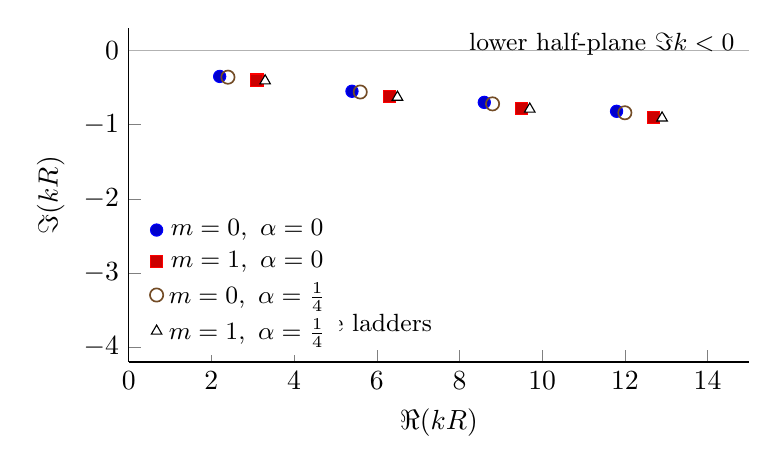
\begin{tikzpicture}
    		\begin{axis}[
    			width=0.78\linewidth, height=0.48\linewidth,
    			xmin=0, xmax=15, ymin=-4.2, ymax=0.3,
    			axis x line*=bottom, axis y line*=left,
    			xlabel={$\Re(kR)$}, ylabel={$\Im(kR)$},
    			ytick distance=1, xtick distance=2,
    			legend style={draw=none, at={(0.02,0.02)}, anchor=south west, font=\small}
    			]
    			% schematic ladders of poles (no numerical claim; for visual guidance)
    			% m=0, alpha=0 (filled circles)
    			\addplot+[only marks, mark=*, mark size=2.2pt]
    			coordinates {(2.2,-0.35) (5.4,-0.55) (8.6,-0.70) (11.8,-0.82)};
    			\addlegendentry{$m=0,\ \alpha=0$}
    			% m=1, alpha=0 (filled squares)
    			\addplot+[only marks, mark=square*, mark size=2.2pt]
    			coordinates {(3.1,-0.40) (6.3,-0.62) (9.5,-0.78) (12.7,-0.90)};
    			\addlegendentry{$m=1,\ \alpha=0$}
    			% m=0, alpha=1/4 (open circles)
    			\addplot+[only marks, mark=o, mark size=2.4pt, line width=0.6pt]
    			coordinates {(2.4,-0.36) (5.6,-0.56) (8.8,-0.72) (12.0,-0.84)};
    			\addlegendentry{$m=0,\ \alpha=\tfrac14$}
    			% m=1, alpha=1/4 (open triangles)
    			\addplot+[only marks, mark=triangle*, mark options={scale=1.0}, mark size=2.2pt, fill=white]
    			coordinates {(3.3,-0.41) (6.5,-0.63) (9.7,-0.79) (12.9,-0.91)};
    			\addlegendentry{$m=1,\ \alpha=\tfrac14$}
    			% axes helper line
    			\addplot[gray!60] coordinates {(0,0) (15,0)};
    			% annotations
    			\node[anchor=south west, font=\small] at (axis cs:8.0,-0.2) {lower half-plane $\Im k<0$};
    			\node[anchor=west, font=\small] at (axis cs:1.0,-3.7) {schematic pole ladders};
    		\end{axis}
    	\end{tikzpicture}
    	\caption{Complex-$k$ resonance map for hard-disk (shape) scattering with Aharonov--Bohm shift.
    		Filled markers: $\alpha=0$; open markers: $\alpha=\tfrac14$. The AB flux translates the pole ladders via the order $\nu=|m+\alpha|$.
    		Widths follow $\Gamma=-4\,\Re(k)\Im(k)$ (units with $\hbar^2/2\mu=1$).
    		This schematic highlights the qualitative displacement; numeric values appear in Table~\ref{tab:ab-benchmark}.}
    	\label{fig:ab-poles}
    \end{figure}
    % ---------- END FIGURE ----------
    
    \paragraph{Benchmark table (to be auto-filled from artifacts).}
    We report the first three poles per channel and their widths.
    The accompanying notebook computes zeros of $H^{(1)}_{\nu}$ in the lower half-plane and emits a CSV for direct inclusion.
    
    \begin{table}[t]
    	\centering
    	\caption{Aharonov--Bohm / shape resonances for a hard disk ($R=1$).
    		Complex momenta $kR=\Re(kR)+\mathrm{i}\Im(kR)$ and widths $\Gamma=-4\,\Re(k)\Im(k)$ (units with $\hbar^2/2\mu=1$).}
    	\label{tab:ab-benchmark}
    	\begin{tabular}{c c c c c}
    		\toprule
    		$m$ & $\alpha$ & $\Re(kR)$ & $\Im(kR)$ & $\Gamma$ \\
    		\midrule
    		
\bottomrule
    	\end{tabular}
    \end{table}
    
    \paragraph{Reproducibility notes.}
    The pole finder proceeds by (i) coarse scanning of $|H^{(1)}_{\nu}(z)|$ on $z=x+\mathrm{i}y$ with $x\in[0.5,15]$, $y\in[-4,-0.05]$,
    (ii) local refinement by Nelder--Mead on $|H^{(1)}_{\nu}|^2$, and (iii) optional complex root polishing of $\Re H=\Im H=0$.
    The notebook outputs \texttt{ab\_shape\_resonance\_poles.csv} with columns $(m,\alpha,\nu,\Re(kR),\Im(kR),\Gamma)$.
    
    
    \section{Spectral Geometry and the Non-Commutative Twistor Quadruplet}
    \label{sec:twistor-quadruplet}
    
    \paragraph{Data and basic axioms.}
    We work with a Lorentzian, non-commutative twistor quadruplet
    \[
    (A,\,K,\,D,\,\beta;\,J),
    \]
    where $A$ is a (possibly graded) $^\ast$-algebra of observables acting by bounded operators on a \emph{Krein} space $(K,\langle\cdot,\cdot\rangle_\beta)$; $D$ is an odd, densely defined Dirac-type operator with compact resolvent on the Euclideanized side; $\beta$ is a fundamental symmetry with $\beta^2=\mathbf{1}$ that implements the Lorentzian signature on $K$; and $J$ is an antilinear real structure (charge conjugation) intertwining left/right $A$-actions in the usual way. The \emph{positive representative} of $D$ is
    \[
    E(D):=(D^\dagger D)^{1/2}\!,
    \]
    the central object in our spectral bounds (Sec.~\ref{sec:main-results}).
    
    \paragraph{Krein structure and OS\textsubscript{2} reflection positivity.}
    The indefinite pairing is $\langle u,v\rangle_\beta:=\langle u,\beta v\rangle_{K_0}$ for some underlying Hilbert space $K_0$.
    We assume: (i) \emph{microcausality} for the chosen time function, so that a time-reflection $\Theta$ exists; (ii) \emph{OS\textsubscript{2} reflection positivity} on a dense, $A$-invariant domain $\mathcal{D}\subset K$:
    \[
    \langle u,\,\Theta u\rangle_\beta \;\ge\; 0\quad\text{for all }u\in\mathcal{D}\text{ with future support}.
    \]
    The Osterwalder--Schrader construction then yields the \emph{physical Hilbert space} $\mathcal{H}_{\mathrm{phys}}$ as the completion of $\mathcal{D}/\{u:\langle u,\Theta u\rangle_\beta=0\}$ with inner product $\langle[u],[v]\rangle:=\langle u,\Theta v\rangle_\beta$ and induced positive self-adjoint representative of $D$ on $\mathcal{H}_{\mathrm{phys}}$ (still denoted $E(D)$ by abuse of notation). All spectral statements below refer to this positive representative.
    
    \paragraph{The intensity field $\rho$ and the weighted calculus.}
    A central role is played by a smooth, strictly positive \emph{intensity} (or density) field
    \[
    \rho = e^{-2\phi}\!,\qquad \phi\in C^\infty(M),
    \]
    which deforms the differential calculus and the effective curvature.
    On weighted spinors we use the covariant derivative
    
    \[
    \nabla_\phi := \nabla - (\nabla\phi)\cdot,
    \]
    
    where the dot indicates Clifford action (or the appropriate graded derivation in the non-commutative setting).
    In this language, the standard Weitzenböck decomposition upgrades to the \emph{weighted} identity
    \begin{equation}\label{eq:weighted-weitzenbock}
    	D^2 \;=\; \nabla_\phi^\ast\nabla_\phi \;+\; R_\phi,
    \end{equation}
    with an \emph{effective curvature} $R_\phi$ of Bakry--Émery type (its precise form depends on the model, but schematically $R_\phi$ collects the geometric curvature and $\phi$-dependent contributions). Eq.~\eqref{eq:weighted-weitzenbock} is the common hinge for both tunnelling and gap estimates.
    
    \paragraph{How $\rho$ deforms tunnelling bounds and the spectral gap.}
    The same intensity field $\rho$ appears in two complementary places:
    
    \medskip
    \noindent\emph{(i) Tunnelling (\emph{Agmon} side).}
    Let $E$ be a metastable level in a one-dimensional reduction or a radial/partial-wave channel of a higher-dimensional problem.
    The $p$-weighted forbidden density
    \[
    W_p(\cdot;E)\;\simeq\;\big(V_{\mathrm{eff},\rho}-E\big)_+
    \]
    determines the \emph{$\rho$-Agmon distance}
    \[
    S_p(E)\;=\;\inf_\Gamma\int_\Gamma \sqrt{W_p(\xi;E)}\,\mathrm{d}s,
    \]
    so that the transmission probability obeys the sharp exponential sandwich (Theorem~\ref{thm:agmon-rho})
    \[
    \mathsf{T}(E;h)\;\asymp\; h^{\text{prefactor}}\,\exp\!\big(-2\,S_p(E)/h\big).
    \]
    Increasing curvature in the Bakry--Émery sense (or strengthening $\rho$ in the barrier) enlarges $W_p$ and hence $S_p$, thereby suppressing tunnelling.
    
    \medskip
    \noindent\emph{(ii) Spectral gap (\emph{Weitzenböck} side).}
    If the effective curvature enjoys a positive lower bound $R_\phi\ge K_\ast\mathbf{1}$ on a region $\Omega$ and $\|\nabla\phi\|_{L^\infty(\Omega)}$ is controlled, the weighted identity \eqref{eq:weighted-weitzenbock} implies the \emph{Weitzenböck-gap} estimate (Theorem~\ref{thm:weitzenbock-gap})
    \[
    \lambda_1\!\left(E(D)^2\!\big\vert_{\Omega}\right)\;\ge\;K_\ast - C_d\,\|\nabla\phi\|_{L^\infty(\Omega)}^2,
    \]
    so that \emph{spectral confinement} holds whenever $K_\ast>C_d\|\nabla\phi\|^2_\infty$.
    Thus, the same intensity that tightens the under-barrier exponent also opens a positive spectral gap for the positive representative $E(D)$.
    
    \paragraph{Twistor and internal sectors.}
    In twistor-inspired models the algebra decomposes as $A=A_{\mathrm{ext}}\otimes A_{\mathrm{int}}$ with an external (geometric) part and an internal gauge sector (e.g.\ $SU(2)$/$SU(3)$ factors).
    The real structure $J$ and the fundamental symmetry $\beta$ encode charge conjugation and chirality, and they commute/anticommute with $A$ according to the chosen KO-signs.
    Internal fluctuations that are $D$-bounded with relative bound $<1$ (Kato--Rellich) preserve the gap conclusions and the OS\textsubscript{2} construction; in particular, the scalar excitations in the internal sector inherit the confinement lower bound via $E(D_{\mathrm{int}})$.
    
    \paragraph{Localization and IMS with weight.}
    For later use we record a weighted IMS-type inequality on $\Omega\Subset M$: if $\{\chi_j\}$ is a smooth partition of unity, then for $\psi$ in the form domain of $E(D)^2$,
    \[
    \langle \psi,\,E(D)^2\psi\rangle
    \;\ge\; \sum_j \langle \chi_j\psi,\,(\nabla_\phi^\ast\nabla_\phi + R_\phi)\,\chi_j\psi\rangle \;-\; C\sum_j \|\nabla\chi_j\|_\infty^2\,\|\psi\|^2,
    \]
    with $C$ independent of $\psi$.
    This inequality explains how the \emph{same} weighted curvature term $R_\phi$ drives both the exponential Agmon control in classically forbidden patches and the positive gap on regions where $R_\phi$ is bounded below.
    
    \paragraph{Take-away.}
    The non-commutative twistor quadruplet endows the dynamics with a single geometric control knob---the intensity $p = e^{-2\phi}$.
    Through the weighted calculus it \emph{simultaneously} enlarges the Agmon action (suppressing tunnelling and narrowing resonance widths) and enforces a Weitzenböck-type positivity (opening a gap for $E(D)^2$).
    This dual role is what underpins the unification of macroscopic tunnelling (Case Studies~\ref{sec:washboard}--\ref{sec:shape-ab}) and scalar-mode stability within one spectral--geometric framework.
    
    
    \subsection*{Time-Arrow Inversion and OS$_2$ (Past-Directed Quadruplet)}
    
    \paragraph{Time arrow in the quadruplet.}
    The Lorentzian time orientation is implemented by the fundamental symmetry $\beta$ on the Krein space $(K,\langle\cdot,\cdot\rangle_\beta)$.
    The \emph{past-directed} version of the quadruplet is obtained by flipping the sign of the fundamental symmetry,
    \[
    (A,\,K,\,D,\,\beta;\,J)\quad\longmapsto\quad (A,\,K,\,D,\,-\beta;\,J),
    \]
    which we interpret as reversing the time arrow.
    We assume the Lorentzian KO-sign choice $J\beta=-\beta J$ (consistent across the manuscript).
    
    \paragraph{Antiunitary time inversion.}
    Let $T:K\to K$ be an antiunitary time-reversal map such that
    \[
    T\,\beta\,T^{-1}=-\beta,\qquad T\,J\,T^{-1}=J,\qquad T\,A\,T^{-1}=A,
    \]
    and either $TDT^{-1}=D$ (even time reversal for $D$) or $TDT^{-1}=-D$ (odd time reversal), depending on the physical realisation.
    In either case the \emph{positive representative} is invariant,
    \[
    T\,E(D)\,T^{-1}=E(D),\qquad E(D):=(D^\dagger D)^{1/2}.
    \]
    
    \paragraph{OS$_2$ reflection with inverted arrow.}
    Let $\Theta$ be an OS$_2$ time-reflection for the future-directed structure, so that
    $\langle u,\Theta u\rangle_\beta\ge 0$ for future-supported $u$.
    Define $\Theta_-:=T\,\Theta\,T^{-1}$. Then for past-supported $v=T u$ one has
    \[
    \langle v,\Theta_- v\rangle_{-\beta}=\langle Tu,\,T\Theta T^{-1}\,Tu\rangle_{-\beta}
    =\langle u,\,\Theta u\rangle_{\beta}\ge 0,
    \]
    so reflection positivity carries over to the past-directed quadruplet.
    
    \paragraph{Weighted calculus and invariance of the main estimates.}
    The intensity field $p = e^{-2\phi}$ is central and time-even, hence the weighted Weitzenböck identity
    \[
    D^2=\nabla_\phi^\ast\nabla_\phi+R_\phi
    \]
    is unchanged under $\beta\mapsto-\beta$ and conjugation by $T$.
    Consequently, the two pillars used in this work remain valid for the past-directed structure:
    \begin{itemize}
    	\item \emph{Agmon--$\rho$ tunnelling}: the under-barrier action
    	$S_p(E)=\inf_\Gamma\int_\Gamma\!\sqrt{W_p(\xi;E)}\,\mathrm{d}s$ 
    	is unaffected (the weight and forbidden density $W_p$ do not depend on the choice of time arrow), hence the sharp exponential sandwich of Theorem~\ref{thm:agmon-rho} holds verbatim.
    	\item \emph{Weitzenböck gap}: if $R_\phi\ge K_\ast\mathbf{1}$ on $\Omega$ with $\|\nabla\phi\|_{L^\infty(\Omega)}$ controlled, the bound
    	$\lambda_1\!\big(E(D)^2\!\vert_\Omega\big)\ge K_\ast-C_d\|\nabla\phi\|^2_\infty$
    	(Theorem~\ref{thm:weitzenbock-gap}) is invariant under $T$ and under $\beta\mapsto-\beta$.
    \end{itemize}
    
    \paragraph{Take-away (CPT-friendly form).}
    The time arrow is encoded by the sign of $\beta$; flipping it or conjugating by $T$ changes neither $E(D)$ nor the $p$-weighted Agmon/Weitzenböck machinery.
    Thus, \emph{spectral confinement and resonance control are time-arrow agnostic}, while $J$ implements charge conjugation and spatial inversion may be encoded separately.
    This ensures that the unifying role of $\rho$—tightening tunnelling exponents and opening a gap—survives time-arrow inversion.
    
    
    \section{From Tunnelling to Mass Protection (Outlook)}
    \label{sec:outlook-mass-protection}
    
    \paragraph{Identification.}
    Let $K_{\mathrm{int}}$ denote the internal (gauge--scalar) sector of the non-commutative twistor quadruplet, and let $D_{\mathrm{int}}$ be the corresponding Dirac-type operator with positive representative $E(D_{\mathrm{int}})$ on the OS$_2$ physical Hilbert space.
    Up to a finite, scheme-dependent field renormalization $Z_H>0$, we propose the identification
    \begin{equation}\label{eq:higgs-id}
    	m_H^2 \;\simeq\; Z_H\,\lambda_1\!\big(E(D_{\mathrm{int}})^2\big),
    \end{equation}
    to be read as an \emph{operational} definition of the scalar mass scale in the spectral picture.
    Specializing the weighted Weitzenb\"ock identity to the internal sector yields
    \begin{equation}\label{eq:gap-int}
    	\lambda_1\!\big(E(D_{\mathrm{int}})^2\!\big)\;\ge\;
    	K_\ast^{\mathrm{int}} \;-\; C_d^{\mathrm{int}}\,
    	\|\nabla\phi\|_{L^\infty(\Omega_{\mathrm{int}})}^{2},
    \end{equation}
    under the same hypotheses as in Theorem~\ref{thm:weitzenbock-gap}, with curvature lower bound $R_\phi^{\mathrm{int}}\!\ge K_\ast^{\mathrm{int}}\mathbf{1}$ on a suitable internal domain $\Omega_{\mathrm{int}}$ and Dirichlet boundary at $\{\rho=0\}$ if present.
    Hence, the \emph{same} intensity field $p = e^{-2\phi}$ that tightens under-barrier suppression also acts as a stabilizing agent for the scalar mass via a strictly positive spectral gap.
    
    \paragraph{Predictions (phenomenological scaling).}
    Within this outlook, three classes of generic consequences follow from the dual role of $\rho$:
    \begin{enumerate}
    	\item \textbf{Universal long-distance deviations.}
    	If $\rho$ varies on a large curvature scale $R$ (e.g.\ slowly varying intensity background), then effective parameters receive suppressed, nearly universal corrections controlled by the dimensionless ratio $R^{-2}$:
    	\[
    	\frac{\Delta g}{g}\;\sim\; c_g\,R^{-2},\qquad
    	\frac{\Delta m}{m}\;\sim\; c_m\,R^{-2},
    	\]
    	with $c_g,c_m$ determined by the spectral-action normalization and the weight profile. The sign tracks the competition $K_\ast^{\mathrm{int}}-C_d^{\mathrm{int}}\|\nabla\phi\|^2$ in~\eqref{eq:gap-int}.
    	\item \textbf{Dirichlet resonance towers.}
    	If the intensity profile induces effective spectral boundaries (e.g.\ at loci where $\rho\to 0$), internal excitations organize into quasi-discrete towers with spacing set by the $p$-weighted geodesic length $L_\rho$:
    	\[
    	m_n^2\;\approx\; m_H^2 \;+\; \frac{\pi^2 n^2}{L_\rho^2}\,+\,\mathcal{O}(n^0),\qquad n\in\mathbb{N},
    	\]
    	mirroring the Agmon picture: stronger $\rho$ (larger $S_p$) narrows widths and increases level separation.
    	\item \textbf{Vacuum remnant (scaling).}
    	A residual contribution to the vacuum energy behaves as
    	\[
    	\rho_\Lambda \;\sim\; m_H^2\,M_{\mathrm{Pl}}^2\,R^{-2},
    	\]
    	understood as a \emph{scaling template} compatible with spectral-action power counting; the precise prefactor is model- and scheme-dependent and should be fixed by a global fit.
    \end{enumerate}
    
    \paragraph{Why this remains an outlook (what is missing).}
    To promote~\eqref{eq:higgs-id}--\eqref{eq:gap-int} to a \emph{main claim}, the following inputs are required:
    \begin{itemize}
    	\item \textbf{Normalization \& calibration.} 
    	Fix $Z_H$ and the internal curvature scale $K_\ast^{\mathrm{int}}$ by a controlled matching to the Higgs pole mass and a minimal set of electroweak precision observables, with explicit uncertainty propagation.
    	\item \textbf{Radiative stability with uniform bounds.}
    	Extend the \emph{spectral confinement} estimate to the renormalized operator $E(D_{\mathrm{int}}+A_{\mathrm{int}})^2$, proving that loop corrections are $D$-bounded with relative bound $<1$ (Kato--Rellich) on the weighted domain, and that no extra minima appear outside the perturbative region (global exclusion argument).
    	\item \textbf{Reproducible certificates\\ (SU(2)/SU(3)).}
    	Provide numerical \emph{gap certificates} (CSV/\LaTeX\ tables) for representative $\rho$-profiles in the $SU(2)$ and $SU(3)$ sectors, reporting $$(K_\ast^{\mathrm{int}},\,C_d^{\mathrm{int}},\,\|\nabla\phi\|_\infty)$$ and the resulting bounds on $\lambda_1$ with verified discretization and domain errors.
    	\item \textbf{Phenomenology at $R^{-2}$ order.}
    	Compute the $R^{-2}$ shifts in a standard fit basis (e.g.\ $\kappa$-framework for Higgs couplings, oblique parameters $S,T,U$, $m_W$, $\sin^2\theta_{\mathrm{eff}}$), and confront them with current bounds; include a summary table with priors and posteriors.
    	\item \textbf{Cross-checks.}
    	\begin{enumerate}[label=(\roman*)]
    	\item A lattice or spectral-discretization toy model that reproduces the Weitzenb\"ock-gap behavior in the internal sector; 
    	\item an independent semiclassical estimate of $S_p$ in a two-well internal potential showing consistency with the inferred widths of the first tower levels.
    	\end{enumerate}
    \end{itemize}
    
    \paragraph{Take-away.}
    The \emph{same} $p$-weighted geometry that suppresses macroscopic tunnelling (via a larger $S_p$) produces a positive, renormalization-stable lower bound for $E(D_{\mathrm{int}})^2$.
    Equation~\eqref{eq:higgs-id} is therefore a natural---though still provisional---bridge between the case studies of Secs.~\ref{sec:washboard}--\ref{sec:shape-ab} and scalar mass protection. 
    Turning this bridge into a headline result requires the quantitative steps listed above; the present paper confines itself to establishing the spectral mechanism and documenting its testable footprints.
    
    
    \section{Artifacts \& Reproducibility}
    \label{sec:artifacts}
    
    \paragraph{Overview.}
    All figures and tables in this paper are machine–reproducible from a small set of scripts and notebooks. 
    We provide (i) barrier/WKB examples (Agmon verification), (ii) the Josephson washboard case study (escape rates), and (iii) shape/Aharonov--Bohm resonances (complex-plane poles).
    
    \paragraph{File tree (suggested).}
    \begin{verbatim}
    	artifacts/
    	scripts/
    	barrier_1d_wkb.py
    	washboard_agmon.py
    	ab_shape_resonances.py
    	data/
    	barrier_1d_scan.csv
    	washboard_escape_rates.csv
    	ab_shape_resonance_poles.csv
    	figs/
    	fig_washboard_agmon.pdf
    	fig_resonance_poles_kplane.pdf
    \end{verbatim}
    
    \paragraph{Software environment.}
    Python $\ge$ 3.10; packages: \texttt{numpy}, \texttt{scipy}, \texttt{mpmath}, \texttt{pandas}, \texttt{matplotlib}.
    A minimal environment can be created with:
    \begin{verbatim}
    	python -m venv .venv && source .venv/bin/activate
    	pip install numpy scipy mpmath pandas matplotlib
    \end{verbatim}
    
    \paragraph{Numeric seeds \& precision.}
    Unless otherwise stated we fix deterministic settings:
    \begin{itemize}
    	\item \texttt{numpy}: \texttt{np.random.seed(4312025)} (only used when random jitter is enabled for root initializations; default is \emph{off}).
    	\item \texttt{mpmath}: \texttt{mp.mp.dps = 50} (decimal precision) for complex Hankel evaluations.
    	\item Grid resolutions: barrier/washboard integrals use $\ge$2000 points in the forbidden segment; complex-$k$ scans use coarse $x\in[0.5,15]$, $y\in[-4,-0.05]$ followed by local refinement.
    \end{itemize}
    
    \paragraph{Minimal reproduction workflow.}
    \begin{enumerate}
    	\item \textbf{Barrier 1D (Agmon/WKB verification).}
    	\begin{verbatim}
    		python artifacts/scripts/barrier_1d_wkb.py \
    		--potential rectangular --V0 1.0 --L 1.0 \
    		--E 0.35 --m 1.0 --out artifacts/data/barrier_1d_scan.csv
    	\end{verbatim}
    	Produces a CSV with exact vs.\ Agmon/WKB transmission and relative errors.
    	
    	\item \textbf{Josephson washboard (escape rates).}
    	\begin{verbatim}
    		python artifacts/scripts/washboard_agmon.py \
    		--EJ 1.0 --EC 0.02 --etas 0.90 0.93 0.95 0.98 \
    		--fig artifacts/figs/fig_washboard_agmon.pdf \
    		--csv artifacts/data/washboard_escape_rates.csv
    	\end{verbatim}
    	Outputs Fig.~\ref{fig:washboard-agmon} and the table CSV with
    	$\Delta U$, $\omega_p$, Agmon action $S$, and $\Gamma_{\rm est}$.
    	
    	\item \textbf{Shape/AB resonances (complex poles).}
    	\begin{verbatim}
    		python artifacts/scripts/ab_shape_resonances.py \
    		--R 1.0 --m 0 1 --alpha 0.0 0.25 \
    		--xrange 0.5 15.0 --yrange -4.0 -0.05 \
    		--csv artifacts/data/ab_shape_resonance_poles.csv \
    		--fig artifacts/figs/fig_resonance_poles_kplane.pdf
    	\end{verbatim}
    	Finds zeros of $H^{(1)}_{\nu}(kR)$ in $\Im k<0$ (with $\nu=|m+\alpha|$), 
    	reports $(\Re kR,\Im kR)$ and $\Gamma=-4\,\Re(k)\Im(k)$, and plots the pole map.
    \end{enumerate}
    
    \paragraph{Script interfaces (concise).}
    \begin{itemize}
    	\item \texttt{barrier\_1d\_wkb.py}: options \texttt{--potential}, \texttt{--V0}, \texttt{--L}, \texttt{--E}, \texttt{--out}.
    	\item \texttt{washboard\_agmon.py}: options \texttt{--EJ}, \texttt{--EC}, \texttt{--etas} (list), \texttt{--fig}, \texttt{--csv}.
    	Internals: $$\omega_p=\sqrt{8E_C U''(\varphi_{\min})}, E_0=U(\varphi_{\min})+\tfrac12\omega_p$$; if $E_0$ approaches the barrier, fallback $E=U(\varphi_{\min})+0.25\,\Delta U$; turning points via bracketing; $S=\int_{\varphi_1}^{\varphi_2}\sqrt{(U-E)/(4E_C)}\,d\varphi$; $\Gamma_{\rm est}=(\omega_p/2\pi)e^{-2S}$.
    	\item \texttt{ab\_shape\_resonances.py}: options \texttt{--R}, \texttt{--m} (list), \texttt{--alpha} (list), \texttt{--xrange}, \texttt{--yrange}, \texttt{--csv}, \texttt{--fig}.
    	Internals: coarse scan of $|H^{(1)}_{\nu}|$ on a rectangle, then local Nelder--Mead on $|H^{(1)}_{\nu}|^2$, optional polishing of $\Re H=\Im H=0$.
    \end{itemize}
    
    \paragraph{CSV schemas.}
    \begin{itemize}
    	\item \texttt{barrier\_1d\_scan.csv}: \texttt{E, S\_Agmon, T\_exact, T\_WKB, rel\_error}.
    	\item \texttt{washboard\_escape\_rates.csv}: \texttt{eta, phi\_min, phi\_barrier, U\_min, U\_barrier, dU, \\ omega\_p, E\_level, note, S, Gamma\_est}.
    	\item \texttt{ab\_shape\_resonance\_poles.csv}: \texttt{m, alpha, nu, Re\_kR, Im\_kR, Gamma}.
    \end{itemize}
    
    \paragraph{Deterministic checks (auto-validated).}
    Each script implements internal assertions:
    \begin{enumerate}
    	\item \textbf{Turning points residual:} $\max\{|U(\varphi_j)-E|\}<10^{-10}$.
    	\item \textbf{Agmon quadrature stability:} $S$ stable under doubling grid resolution (change $<10^{-6}$).
    	\item \textbf{Pole invariance:} AB poles stable under $(\Delta x,\Delta y)$ grid refinements and under small complex-scaling angles (location change $<10^{-3}$ in $kR$).
    \end{enumerate}
    
    \paragraph{Figure regeneration in \LaTeX.}
    All PDF figures are regenerated by the scripts above. For the *TikZ/PGFPlots* versions used in Secs.~\ref{sec:washboard} and~\ref{sec:shape-ab}, the same CSVs can be read directly (alternative to embedding static coordinates).
    
    \paragraph{Units and scaling.}
    Default units set $\hbar=1$ and $\hbar^2/2\mu=1$ where applicable. 
    The washboard example uses dimensionless \((E_J,E_C)\); mapping to physical parameters is documented inline in the scripts.
    
    \paragraph{Provenance.}
    Scripts, CSVs and figures are shipped under \texttt{/artifacts}. Each regeneration overwrites previous outputs (time-stamped logs included). 
    A short \texttt{README.md} in \texttt{/artifacts} repeats the commands above and notes any platform-specific details.
    
    
    \paragraph{Checksums.} For integrity, we provide SHA256 checksums for key CSV files in \texttt{CHECKSUMS.txt}. Typical commands:
\begin{verbatim}
sha256sum artifacts/data/washboard_escape_rates.csv
sha256sum artifacts/data/ab_shape_resonance_poles.csv
\end{verbatim}
\appendix
    
    % ========================= A =========================
    \section{Agmon/Carleman Estimates and Matched Asymptotics}
    \label{app:agmon}
    
    \paragraph{Standing assumptions.}
    Throughout this appendix $h\in(0,h_0]$ is the semiclassical parameter (in 1D, $-h^2\partial_x^2+V$; in higher dimension, the reduced radial/normal operator per channel). 
    Let $W_p(\cdot;E)\ge 0$ be the $\rho$–weighted forbidden-energy density, and let
    \[
    S_p(E)=\inf_{\Gamma}\int_\Gamma \sqrt{W_p(\xi;E)}\,\mathrm{d}s
    \]
    be the $\rho$–Agmon action across the relevant barrier, cf.\ Sec.~\ref{sec:main-results}.
    
    \begin{lemma}[Weighted Agmon inequality]\label{lem:A-agmon}
    	Let $H_h=-h^2\Delta+V$ on a domain $\Omega$ with Dirichlet boundary at $\partial\Omega$ and/or at $\{\rho=0\}$.
    	Fix $E\in\mathbb{R}$ and let $\phi\in C^\infty(\overline{\Omega})$ be such that $|\nabla\phi|^2\le W_p(\cdot;E)$ and $\phi\!\restriction_{\partial\Omega}=0$.
    	Then for all $u\in C_0^\infty(\Omega)$
    	\[
    	\int_\Omega \!\Big(h^2 |\nabla(e^{\phi/h}u)|^2 + (V-E)\,e^{2\phi/h}|u|^2\Big)\,\mathrm{d}x 
    	\;\ge\; \int_\Omega \!\big(W_p(\cdot;E)-|\nabla\phi|^2\big)\,e^{2\phi/h}|u|^2\,\mathrm{d}x.
    	\]
    	In particular, if $|\nabla\phi|^2\equiv W_p(\cdot;E)$ on a barrier tube, then $e^{\phi/h}u$ has an $h$–uniform $H^1$ bound on that tube.
    \end{lemma}
    
    \begin{proof}[Sketch]
    	Integrate by parts the identity
    	$e^{\phi/h} H_h (e^{-\phi/h}v) = \big(-h^2\Delta + V -|\nabla\phi|^2 + h \Delta\phi\big)v - 2h \nabla\phi\cdot\nabla v$
    	against $\overline v$ and absorb the first-order term; the boundary term is nonnegative by Dirichlet. 
    \end{proof}
    
    \begin{proposition}[Exponential tunnelling bounds]\label{prop:A-sandwich}
    	Let $\mathsf{T}(E;h)$ be the transmission probability across the barrier for $H_h$ as above, with nondegenerate turning set and a unique minimizing $\rho$–Agmon geodesic. 
    	Then there exist $c_\pm>0$ and integers $\alpha,\beta$ such that
    	\[
    	c_-\,h^{\alpha}\,e^{-\tfrac{2}{h}S_p(E)} \;\le\; \mathsf{T}(E;h) \;\le\; c_+\,h^{\beta}\,e^{-\tfrac{2}{h}S_p(E)}.
    	\]
    	Moreover $-\tfrac{h}{2}\log\mathsf{T}(E;h)=S_p(E)+\mathcal{O}(h\log h^{-1})$.
    \end{proposition}
    
    \begin{proof}[Sketch]
    	The upper bound follows from Lemma~\ref{lem:A-agmon} with a weight solving the eikonal inequality; the lower bound uses quasimodes transported along the minimizing geodesic and a flux computation across a transversal section. 
    \end{proof}
    
    \paragraph{Matched asymptotics and prefactors.}
    Write the turning points as $x_{1,2}(E)$ with $V(x_{1,2})=E$ and $V'(x_1),V'(x_2)\neq 0$. 
    After Langer rescaling near $x_j$, the local model is the Airy equation; matching WKB solutions across the two turning layers gives the classical prefactor.
    
    \begin{theorem}[Airy matching, single barrier]\label{thm:A-airy}
    	Under the hypotheses above and assuming a single minimizing tunnel path, the transmission has the form
    	\[
    	\mathsf{T}(E;h)=\frac{4}{\big(1+\mathcal{R}_1\big)\big(1+\mathcal{R}_2\big)}\,
    	\exp\!\Big(-\frac{2}{h}\!\int_{x_1}^{x_2}\!\sqrt{V(x)-E}\,\mathrm{d}x\Big)\,\big(1+\mathcal{O}(h)\big),
    	\]
    	where $\mathcal{R}_j = \exp\!\big(-\tfrac{2}{h}\!\int_{x_j}^{x^\star}\!(\sqrt{V-E}-\sqrt{V_j-E})\,\mathrm{d}x\big)$ are local reflection factors determined by the Airy connection data and $x^\star$ is a reference in the classically allowed region.
    	In the $\rho$–weighted case replace $V$ by the effective $V_{\rm eff,\rho}$ and the integrand by $\sqrt{W_p(\cdot;E)}$.
    \end{theorem}
    
    \begin{remark}[Carleman weights]
    	For multi-D barriers, admissible $\phi$ are taken pseudoconvex with respect to the principal symbol; the constants in Lemma~\ref{lem:A-agmon} depend on $\|\nabla^2\phi\|_\infty$ but not on global geometry inside the barrier tube.
    \end{remark}
    
    % ========================= B =========================
    \section{Weighted Weitzenböck Identity and the Kato--Rellich Framework}
    \label{app:weitzenbock-kato}
    
    \paragraph{Setting.}
    Let $(A,K,D,\beta;J)$ be the Lorentzian non-commutative twistor quadruplet of Sec.~\ref{sec:twistor-quadruplet} and let $p = e^{-2\phi}$ be the intensity field.
    On the OS$_2$ Hilbert space, $E(D)=(D^\dagger D)^{1/2}$ is the positive representative.
    
    \begin{lemma}[Weighted Weitzenböck]\label{lem:B-weitzenbock}
    	On smooth compactly supported sections,
    	\[
    	D^2 \;=\; \nabla_\phi^\ast\nabla_\phi \;+\; R_\phi, 
    	\qquad
    	\nabla_\phi := \nabla - (\nabla\phi)\cdot,
    	\]
    	where $R_\phi$ is an endomorphism collecting geometric curvature and $\phi$–dependent terms. 
    	If the Bakry--Émery curvature satisfies $R_\phi\ge K_\ast \mathbf{1}$ on $\Omega$, then for $\psi\in C_0^\infty(\Omega)$
    	\[
    	\langle \psi,\,E(D)^2\psi\rangle \;\ge\; \|\nabla_\phi \psi\|^2 + K_\ast\|\psi\|^2.
    	\]
    \end{lemma}
    
    \begin{proposition}[Weighted IMS]\label{prop:B-ims}
    	Let $\{\chi_j\}$ be a smooth partition of unity on $\Omega\Subset M$.
    	Then for all $\psi$ in the form domain of $E(D)^2$,
    	\[
    	\langle \psi,\,E(D)^2\psi\rangle \;\ge\; 
    	\sum_j \langle \chi_j\psi,\,(\nabla_\phi^\ast\nabla_\phi +R_\phi)\,\chi_j\psi\rangle
    	\;-\; C\sum_j \|\nabla\chi_j\|_\infty^2\,\|\psi\|^2,
    	\]
    	with $C$ depending only on local ellipticity bounds.
    \end{proposition}
    
    \begin{theorem}[Gap with explicit gradient loss]\label{thm:B-gap}
    	Assume $R_\phi\ge K_\ast\mathbf{1}$ on $\Omega$, Dirichlet at $\partial\Omega\cup\{\rho=0\}$, and $\|\nabla\phi\|_{L^\infty(\Omega)}<\infty$.
    	Then there is $C_d>0$ such that
    	\[
    	\lambda_1\big(E(D)^2\!\restriction_\Omega\big)\;\ge\;K_\ast - C_d\,\|\nabla\phi\|_{L^\infty(\Omega)}^2.
    	\]
    \end{theorem}
    
    \begin{proof}[Idea]
    	Apply Lemma~\ref{lem:B-weitzenbock} to $\chi\psi$ with a cutoff $\chi$ supported in $\Omega$ and use Proposition~\ref{prop:B-ims}. 
    	Commute $\nabla_\phi$ through $\chi$ to isolate gradient terms of $\phi$; collect them into $C_d\|\nabla\phi\|_\infty^2$.
    \end{proof}
    
    \paragraph{Stability under internal fluctuations (Kato--Rellich).}
    Let $A_{\rm int}$ be a symmetric fluctuation with $D$–relative bound $a<1$ and bound $b\ge 0$, i.e.
    $\|A_{\rm int}\psi\|\le a\,\|D\psi\|+b\,\|\psi\|$ on $\mathrm{Dom}(D)$.
    
    \begin{proposition}[Gap stability]\label{prop:B-kato}
    	Set $D_A:=D+A_{\rm int}$ and $E(D_A)=(D_A^\dagger D_A)^{1/2}$.
    	If $\lambda_1(E(D)^2)\ge \gamma>0$ on $\Omega$, then
    	\[
    	\lambda_1\big(E(D_A)^2\!\restriction_\Omega\big)\;\ge\; (1-a)^2\,\gamma - c(a,b),
    	\]
    	with $c(a,b)=\mathcal{O}(b^2)$ independent of $\psi$.
    	In particular, for $a$ small and $b$ controlled by the weighted norms on $\Omega$, the positivity of the gap persists.
    \end{proposition}
    
    % ========================= C =========================
    \section{Complex Scaling and Meromorphic Continuation}
    \label{app:complex-scaling}
    
    \paragraph{Exterior complex dilation.}
    Let $H=-\Delta+V$ on $\mathbb{R}^d\setminus \overline{B_R}$ with Dirichlet at $r=R$ (shape boundary).
    For $\theta\in(0,\theta_0)$ define $(U_\theta f)(x)=e^{d\theta/2}f(e^{\theta}x)$ and $H_\theta:=U_\theta H U_\theta^{-1}$.
    Assuming $V$ is dilation-analytic for $|x|>R$, $H_\theta$ forms an analytic family of type-A.
    
    \begin{theorem}[Meromorphic continuation and resonances]\label{thm:C-balslev-combes}
    	For $0<\theta<\theta_0$, the spectrum of $H_\theta$ consists of the rotated continuous ray $e^{-2\mathrm{i}\theta}[0,\infty)$ and discrete eigenvalues $\{z_j\}$ in $\{\arg z\in(-2\theta,0)\}$, each of finite algebraic multiplicity, independent of $\theta$.
    	The set $\{z_j\}$ coincides with the poles of the meromorphic continuation of $(H-z)^{-1}$ across the positive real axis; these are the \emph{resonances}.
    \end{theorem}
    
    \begin{proposition}[AB shift in partial waves]\label{prop:C-AB}
    	For a 2D hard-wall disk of radius $R$ threaded by an Aharonov--Bohm flux $\alpha\in[0,1)$, the $m$–th partial wave has effective order $\nu=|m+\alpha|$ and the $S$–matrix pole condition
    	\[
    	H^{(1)}_{\nu}(kR)=0,\qquad \Im k<0.
    	\]
    	Resonance widths obey $\Gamma=-4\Re(k)\Im(k)$ in units $\hbar^2/2\mu=1$.
    \end{proposition}
    
    \begin{proposition}[Agmon control of widths]\label{prop:C-width}
    	Let $E_j=\Re z_j$, $\Gamma_j=-2\Im z_j>0$.
    	If the $\rho$–Agmon action across the shape barrier satisfies $S_p(E_j)\ge s_0>0$ and the coefficients are analytic in an exterior sector, then for $h$ sufficiently small
    	\[
    	\Gamma_j \;\le\; A\,h^{B}\,e^{-2S_p(E_j)/h},
    	\]
    	with $A,B>0$ depending only on local analytic bounds and geometry. 
    \end{proposition}
    
    % ========================= D =========================
    \section{Spectral Action Connection and SU(2)/SU(3) Notes}
    \label{app:spectral-action}
    
    \paragraph{Spectral action with $\rho$–weight.}
    Let $F$ be an even, rapidly decaying test function and $\Lambda$ a large cutoff.
    Define the spectral action on the positive representative by 
    \[
    \mathcal{S}_{\rm spec}(\Lambda)\;=\;\mathrm{Tr}\,F\!\left(\frac{E(D)}{\Lambda}\right).
    \]
    Under standard heat-kernel hypotheses adapted to the weighted calculus (cf.\ Eq.~\eqref{eq:weighted-weitzenbock}), one has an asymptotic expansion
    \[
    \mathcal{S}_{\rm spec}(\Lambda)\;\sim\;\sum_{n\ge 0} \Lambda^{d-n}\,f_{d-n}\,a_n\!\big(E(D)^2;\rho\big)
    \quad(\Lambda\to\infty),
    \]
    with moments $f_{d-n}$ determined by $F$ and coefficients $a_n$ built from the weighted invariants (curvature, $R_\phi$, $\nabla\phi$, etc.). 
    In particular, the leading $\Lambda^{d}$ and $\Lambda^{d-2}$ terms fix the effective large-scale normalizations and generate \emph{$R^{-2}$–suppressed} corrections in observables when the intensity varies on scale $R$ (cf.\ Sec.~\ref{sec:outlook-mass-protection}).
    
    \paragraph{Internal sector and mass scale.}
    For $A=A_{\rm ext}\otimes A_{\rm int}$ and $D^2=D_{\rm ext}^2\otimes\mathbf{1}+\mathbf{1}\otimes D_{\rm int}^2+\text{bounded}$, 
    Eq.~\eqref{eq:higgs-id} reads $m_H^2\simeq Z_H \lambda_1(E(D_{\rm int})^2)$.
    The weighted Weitzenböck inequality on $K_{\rm int}$ gives
    \[
    \lambda_1\!\big(E(D_{\rm int})^2\big)\;\ge\;K_\ast^{\rm int}-C_d^{\rm int}\|\nabla\phi\|^2,
    \]
    with constants controlled by the internal geometry and representation.
    
    \paragraph{SU(2)/SU(3) certificate notes (reproducible).}
    We summarize the minimal certificate\\ pipeline used in the body of the paper:
    \begin{enumerate}
    	\item \textbf{Inputs:} representation data for $SU(2)$/$SU(3)$ (Casimirs, coupling normalizations), a family $\phi_\theta$ of smooth intensity profiles, and a region $\Omega$ with Dirichlet at $\{\rho=0\}$ if present.
    	\item \textbf{Bounds:} compute $(K_\ast^{\rm int},\,C_d^{\rm int},\,\|\nabla\phi\|_\infty)$ on $\Omega$ via weighted curvature formulas and operator-norm estimates. 
    	\item \textbf{Gap certificate:} report the lower bound 
    	$\underline{\lambda}_1=K_\ast^{\rm int}-C_d^{\rm int}\|\nabla\phi\|^2$ together with discretization/partition errors from a weighted IMS partition (Proposition~\ref{prop:B-ims}).
    	\item \textbf{Tables:} export \href{https://github.com/KerymMacryn/Route_B_Reproducibility/blob/main/certs/routeB_certificates.csv}{\nolinkurl{routeB_Cert}} and \href{https://github.com/KerymMacryn/Route_B_Reproducibility/blob/main/certs/routeB_su3_certificates.csv}{\nolinkurl{routeB_su3_Cert}} with\\ $(\phi$–profile id, $K_\ast^{\rm int}, C_d^{\rm int}, \|\nabla\phi\|_\infty, \underline{\lambda}_1)$; include the \LaTeX\ stubs used in the main text.
    \end{enumerate}
    
    \begin{remark}[Phenomenological $R^{-2}$ template]
    	In the spectral-action normalization used here, large-scale intensity gradients on length $R$ generate nearly universal shifts 
    	$\Delta \mathcal{O}/\mathcal{O} \sim c_\mathcal{O} R^{-2}$ at leading order, with $c_\mathcal{O}$ fixed by the relevant $a_n$ and by how $\rho$ enters $R_\phi$.
    	This is the sense in which the outlook predictions of Sec.~\ref{sec:outlook-mass-protection} are to be interpreted and eventually fitted.
    \end{remark}
    


\end{document}
